%%%%%%%%%%%%%%%%%%%%%%%%%%%%%%%%%%%%%%%%%%%%%%%%%%%%%%%%%%%%%%%%%%%%%%%%%%%

\documentclass[a4paper,oneside,12pt]{article}
\usepackage{mystyle}

\begin{document}

\title{\Large\bf Quadratic functions}
\author{%%
  Minh Van Nguyen \\
  \url{mvngu@gmx.com}
}
\date{\today}
\maketitle

\begin{packeditem}
\item General quadratic function.

\item Graph of quadratic function.

\item Factoring quadratic function.

\item Completing the square.

\item Application: gravity and displacement of projectile.

\item Area under a quadratic function.
\end{packeditem}


%%%%%%%%%%%%%%%%%%%%%%%%%%%%%%%%%%%%%%%%%%%%%%%%%%%%%%%%%%%%%%%%%%%%%%%%%%%

\section{General form}

A \emph{quadratic function} is an equation of the form
%%
\begin{equation}
\label{eqn:general_quadratic_function}
f(x)
=
ax^2 + bx + c
\end{equation}
%%
where $\triple{a}{b}{c} \in \RR$ are known constants and $x$ is a
variable that can be any real number.  What does the function $f(x)$
look like?

As an example, set $a = 1$ and $b = c = 0$ in
\Equation{eqn:general_quadratic_function} so that you have
$f(x) = x^2$.  Let's calculate the function value for
$x = \sextuple{-4}{-3}{-2}{2}{3}{4}$.  Note that you have
\[
f(2) = f(-2) = 4,
%%
\quad
%%
f(3) = f(-3) = 9,
%%
\quad
%%
f(4) = f(-4) = 16.
\]
Plot these points on one set of coordinate axes and draw a line
through the points to get the graph in \Figure{fig:quadratic_a_1}.
Note that $f(0) = 0$ so the graph of $f(x) = x^2$ touches the origin.
The general shape of the graph of
\Equation{eqn:general_quadratic_function} looks like the beak of a
duck~(or some other bird) and the usual name for this is a
\emph{parabola}.

\begin{figure}[!htbp]
\centering
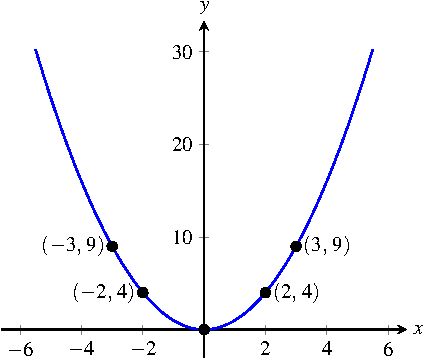
\includegraphics[scale=1.2]{image/07/a-1.pdf}
\caption{%%
  A graph of the function $f(x) = x^2$.  The general shape of the
  graph is called a \emph{parabola}.
}
\label{fig:quadratic_a_1}
\end{figure}
\end{document}
